\documentclass[a4paper]{report}
\usepackage[utf8]{inputenc}
\usepackage[T1]{fontenc}
\usepackage[swissgerman]{babel}
\usepackage[left=2cm,right=1.5cm,top=1.5cm,bottom=1.5cm]{geometry}
\usepackage{amssymb}
\usepackage{ragged2e}
\usepackage{titlesec}
\usepackage{booktabs}
\usepackage{svg}
\usepackage{transparent}
\usepackage{float}
\usepackage{hyperref}
\usepackage[many]{tcolorbox}
\usepackage{epigraph}
\usepackage{listings}

\lstloadlanguages{Java,Ruby}
\lstdefinestyle{fmo}{
  keywordstyle=\color{blue},
  identifierstyle=\bfseries\color{black},
  frame=single,
  basicstyle=\footnotesize\ttfamily,
  showstringspaces=false,
  keepspaces=true,
}
\lstset{style=fmo}

\setsvg{inkscape=inkscape -z -D,svgpath=__src/svg/}

\setlength\parindent{0pt}
\linespread{1.3}

\titleformat{\chapter}[display]
{\normalfont\huge\bfseries}{\chaptertitlename\ \thechapter}{20pt}{\Huge}
\titlespacing*{\chapter}{0pt}{0pt}{40pt}

%\renewcommand{\labelenumi}{\alph{enumi}.}

\newcommand{\pro}[1]{\item [pro]#1}
\newcommand{\con}[1]{\item [con]#1}

\newtcolorbox{caveat}[1][]{
  breakable,
  freelance,
  title=CAVEAT: #1,
  colback=white,
  colbacktitle=white,
  coltitle=black,
  fonttitle=\bfseries,
  bottomrule=0pt,
  boxrule=0pt,
  colframe=white,
  overlay unbroken and first={
    \draw[red!75!black,line width=3pt]
    ([xshift=5pt]frame.north west) -- 
    (frame.north west) -- 
    (frame.south west);
    \draw[red!75!black,line width=3pt]
    ([xshift=-5pt]frame.north east) -- 
    (frame.north east) -- 
    (frame.south east);
  },
  overlay unbroken app={
    \draw[red!75!black,line width=3pt,line cap=rect]
    (frame.south west) -- 
    ([xshift=5pt]frame.south west);
    \draw[red!75!black,line width=3pt,line cap=rect]
    (frame.south east) -- 
    ([xshift=-5pt]frame.south east);
  },
  overlay middle and last={
    \draw[red!75!black,line width=3pt]
    (frame.north west) -- 
    (frame.south west);
    \draw[red!75!black,line width=3pt]
    (frame.north east) -- 
    (frame.south east);
  },
  overlay last app={
    \draw[red!75!black,line width=3pt,line cap=rect]
    (frame.south west) --
    ([xshift=5pt]frame.south west);
    \draw[red!75!black,line width=3pt,line cap=rect]
    (frame.south east) --
    ([xshift=-5pt]frame.south east);
  },
}

\newtcolorbox{additional}[1][]{
  breakable,
  freelance,
  title=Additional Resources: #1,
  colback=white,
  colbacktitle=white,
  coltitle=black,
  fonttitle=\bfseries,
  bottomrule=0pt,
  boxrule=0pt,
  colframe=white,
  overlay unbroken and first={
    \draw[green!75!black,line width=3pt]
    ([xshift=5pt]frame.north west) -- 
    (frame.north west) -- 
    (frame.south west);
    \draw[green!75!black,line width=3pt]
    ([xshift=-5pt]frame.north east) -- 
    (frame.north east) -- 
    (frame.south east);
  },
  overlay unbroken app={
    \draw[green!75!black,line width=3pt,line cap=rect]
    (frame.south west) -- 
    ([xshift=5pt]frame.south west);
    \draw[green!75!black,line width=3pt,line cap=rect]
    (frame.south east) -- 
    ([xshift=-5pt]frame.south east);
  },
  overlay middle and last={
    \draw[green!75!black,line width=3pt]
    (frame.north west) -- 
    (frame.south west);
    \draw[green!75!black,line width=3pt]
    (frame.north east) -- 
    (frame.south east);
  },
  overlay last app={
    \draw[green!75!black,line width=3pt,line cap=rect]
    (frame.south west) --
    ([xshift=5pt]frame.south west);
    \draw[green!75!black,line width=3pt,line cap=rect]
    (frame.south east) --
    ([xshift=-5pt]frame.south east);
  },
}

\title{POSA 1 - HS2015}

\author{Valentin \textsc{Meier}\\\\Vorlage von Felix \textsc{Morgner}}

\date{\today}

\begin{document}

\maketitle
\clearpage
\vspace*{\fill}
  \epigraph{Sometimes the questions are complicated and the answers are simple.}{Dr. Seuss}
\vfill
\clearpage

\setcounter{tocdepth}{0}
\tableofcontents

\chapter{Layers}

\section{Summary}
Das Layer Pattern hilft Applikationen zu strukturieren, welche in Gruppen von Teilaufgaben zerteilt werden können so dass, jede Gruppe auf einem bestimmten Abstraktionslevel ist.
\section{Context}
Ein grosses System das Zerlegung benötigt.

\section{Problem}
Ein grosses System mit Low- und Highlevel Problemen hat zu wenig Struktur. Die Highlevel-Probleme bauen dabei auf den Lowlevel-Problemen auf. Es ist schwer Wartbar und die Aufgaben und Grenzen zwischen den Komponenten sind ungenau.

Ein mögliches Beispiel für ein solches System ist ein Netzwerk. Dabei ist ein Lowlevel-Problem: \textit{"Wie bringe ich Daten von A nach B?"} und ein Highlevel-Problem: \textit{"Wie ordne ich verschiedene Pakete einer logischen Session zu?"}

\section{Solution}
Das System wird in beliebig viele Layer aufgeteilt. Die Layer bauen aufeinander auf, wobei der höchste Layer den höchsten Abstraktionsgrad hat. Alle Komponenten mit dem selben Abstrationsgrad befinden sich auf dem selben Layer. Jedem Layer werden bestimmte Aufgaben zugewiesen. Er nutzt jeweils die Services des eins tieferen Layers. \\\\
Bei vielen Komponenten pro Layer wird je Layer ein Interface Objekt definiert welches mit den anderen Layern kommuniziert. Meist wird aus einem Request (Zugriff von Oben nach Unten) mehrere je tiefer der Request in den Layern nach unten wandert. Das Umgekehrte gilt bei einer Notification (Zugriff von Unten nach Oben).
Die folgenden Schritte beschreiben einen schrittweisen Ansatz zur Definition einer Layer Architektur. Dies ist nicht immer die beste Lösung. Es sind auch nicht alle Schritte zwingend notwendig. Vorgehen:
\begin{enumerate}
	\item Abstraktionskriterien definieren (Wie die Layer sich abgrenzen)
	\item Anzahl Abstraktionslevel definieren
	\item Layers benennen und Tasks zuteilen
	\item Services pro Layer spezifizieren
	\item 1.-4. zur Verfeinerung wiederholen
	\item Ein Interface pro Layer definieren, eventuell Facade Pattern anwenden
	\item Layer im Innern strukturieren (Bridge/Strategy Pattern)
	\item Kommunikation zwischen benachbarten Layern spezifizieren
	\item Benachbarte Layer entkuppeln (Bsp. One-Way Coupling/Retour mit Callbacks)
	\item Error Handling Strategie entwickeln. Entweder im Layer behandeln oder an den nächst höheren weitergeben. Faustregel:Am besten am tiefstmöglichen Layer behandeln.
\end{enumerate}
Es gibt noch zwei weitere Varianten des Layer Pattern:
\begin{description}
	\item[Relaxed Layered System] Layer können Services aller unterliegenden Layer benutzen. Mehr Flexibilität und Performance, jedoch schlechtere Wartbarkeit.
	\item[Layering through inheritance] Für OO-Systeme. Lower Layer als base classes. Höhere Layer erben von diesen. So können höhere Layer Funktionalität von tieferen ihren Bedürfnissen anpassen.
\end{description}

\subsection{Structure}

\begin{figure}[H]
  \centering
  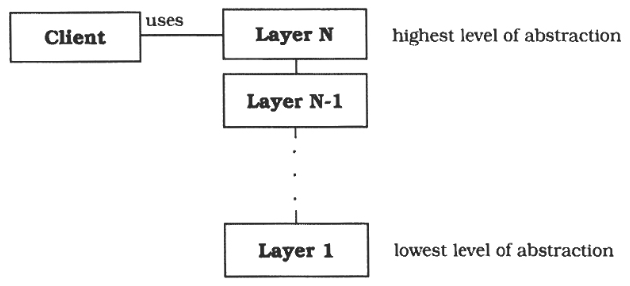
\includegraphics[width=0.8\textwidth]{figures/00-layers-1}
  \caption{Illustration des Layer-Patterns}
\end{figure}

\section{Consequences}
\begin{itemize}
    \pro{Wiederverwendbarkeit von Layern}
    \pro{Austauschbarkeit von Layern}
    \pro{Support für Standardisierung}
    \pro{Dependencies bleiben lokal}
    \con{Tiefere Effizienz}
    \con{Mehr Aufwand}
    \con{Schwierigkeit beim bestimmen der Granularität der Layer}
    \con{Jeder Layer-Übergang schmälert die Performance}
\end{itemize}

\section{Known Uses}
\begin{itemize}
	\item OSI Protocol Stack 
	\item Virtual Machines
	\item APIs
	\item Information Systems
	\item Windows NT
\end{itemize}

\section{Relationships}
\begin{itemize}
	\item \textit{Composite Message} beschreibt eine objekt-orientierte Verschachtelung von Nachrichten, welche durch die Schichten transportiert werden. Eine Composite Message ist ein Paket, welches aus header, payload und eingebetteten Paketen besteht.
	\item \textit{Mikrokernel Architecture} kann als spezialisierte Layer-Architektur angesehen werden.
\end{itemize}

\section{Exam Questions}
\begin{itemize}
  \item Behauptung: Etwas zu bottom-up dekouplung in layer? (Lösung)
    \item Frage: Welches GOF Pattern hilft bei der definierung von Interfaces im Layers Pattern? (Facace Pattern)
\end{itemize}

\chapter{Pipes and Filters}

\section{Summary}
Das "Pipes and Filters" Pattern bietet eine Struktur für Systeme die einen Stream von Daten verarbeiten, dabei wird jeder Verarbeitungsschritt als eine Filterkomponente dargestellt. Die Daten bewegen sich durch Pipes zwischen benachbarten Filtern.  
\section{Context}
Durch das "Pipies and Filters" Pattern werden folgende Forces adressiert: 
\begin{itemize}
	\item Zukünftige Systemerweiterungen sollten durch Austausch oder Neuordnung von Verarbeitungsschritten möglich sein
	\item Kleine Verarbeitungsschritte sind einfacher wiederverwendbar als grosse
	\item Nicht benachbarte Verarbeitungsschritte sollen keine Informationen teilen
	\item Es gibt verschiedene Quellen von Input Daten
	\item Es soll möglich sein Schlussresultate auf verschiedene Arten zu sichern
	\item Explizites Speichern von Zwischenresultate durch User ist fehleranfällig
	\item Man will die Möglichkeit nicht verwerfen, die Arbeitsschritte parallel zu verarbeiten
\end{itemize}


\section{Problem}
Gegeben ist ein System welches einen Stream von Daten verarbeiten muss. Das System wird von mehreren Entwicklern implementiert. Ausserdem lässt sich die generelle Aufgabe des Systems leicht in mehrere Teilaufgaben unterteilen, und die Wahrscheinlichkeit ist hoch, dass sich die Requirements ändern. Die Frage ist nun wie ein solches System designt werden soll damit mehrere Entwickler daran arbeiten können und flexibel auf Änderungen an den Requirements reagiert werden kann.
\section{Solution}
Mittels dem "Pipies and Filters" Pattern werden die Arbeitsschritte eines Systems in mehrere sequentiell verarbeitete Schritte unterteilt. Die Schritte sind durch den Data Flow durch das System verbunden, das heisst, die Output Daten eines Schrittes sind die Input Daten des nächsten. Jeder Arbeitsschritt wird als Filter Komponente implementiert. Ein Filter konsumiert und übermittelt inkrementell. Die Daten Source, die Filter und der Daten "Sink" werden durch sogenannte Pipes verbunden. 

\subsection{Structure}
Filter sind die Verarbeitungseinheiten einer Pipeline. Ein Filter hat drei Aufgaben:
\begin{enumerate}
	\item Anreichern von Daten durch Berechnungen und hinzufügen von Informationen
	\item Verfeinern von Daten durch Konzentration oder Extraktion von Daten
	\item Transformieren von Daten durch Übermittlung in einer anderen Repräsentation
\end{enumerate}
Ein Filter kann durch verschiedene Events ausgelöst werden:
\begin{itemize}
	\item Der darauffolgende Filter pullt die Output Daten
	\item Der vorangehende Filter pushed die Input Daten
	\item Üblicherweise pulling von Input Daten und pushen von Output Daten in einem Loop
\end{itemize}
Bei den ersten beiden Methoden handelt es sich um passive Filter, weil sie darauf warten getriggert zu werden. Bei der dritten Methode handelt es sich um einen aktiven Filter.

%\begin{figure}[H]
%  \centering
%  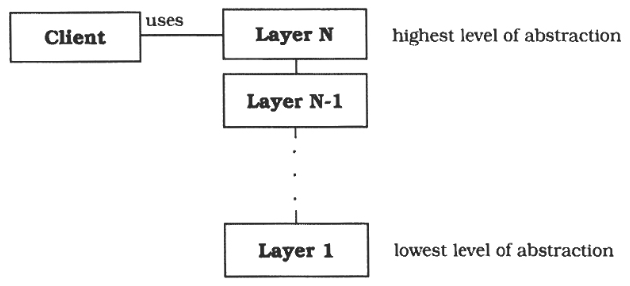
\includegraphics[width=0.8\textwidth]{figures/00-layers-1}
%  \caption{Illustration des Layer-Patterns}
%\end{figure}

\section{Consequences}
\begin{itemize}
    \pro{Keine Speicherung von Zwischenresultaten notwendig, jedoch weiterhin möglich}
    \pro{Flexibilität durch Filteraustausch}
    \pro{Flexibilität durch Neuordnung der Filterreihenfolge}
    \pro{Wiederverwendbarkeit von Filterkomponenten}
    \pro{Schnelles erstellen von Prototypen von Pipelines}
    \pro{Effizienz durch Parallelverarbeitung}
    \con{Teilen von Informationen über den State ist teuer}
    \con{Effizienzsteigerung durch Parallelverarbeitung ist meist eine Illusion}
    \con{Daten Transformations Overhead}
    \con{Error Handling}
    
\end{itemize}

\section{Known Uses}
\begin{itemize}
	\item UNIX
	\item CMS Pipelines
	\item LASSPTools
\end{itemize}

\section{Relationships}
\begin{itemize}
	\item \textit{Layers Pattern} Besser geeignet für Systeme welche zuverlässige Operationen benötigen, da es einfacher ist Error Handling zu implementieren
\end{itemize}

\section{Exam Questions}
\begin{itemize}
  \item Behauptung: dies ist eine Behauptung? (Lösung)
    \item Frage: Dies ist eine Frage? (Lösung)
\end{itemize}

\chapter{Blackboard}

\section{Summary}
Das Blackboard Pattern ist nützlich bei Problemen für die keine deterministischen Lösungsstrategien bekannt sind. Dabei kombinieren mehrere spezialisierte Teilsysteme ihr Wissen um eine annähernde Lösung zu kreieren. 
\section{Context}
Eine unreife Domäne in der keine eindeutige Herangehensweise zu einer Lösung bekannt oder möglich ist.

\section{Problem}
Das Blackboard Pattern kümmert sich um Probleme bei denen es keine praktikable deterministische Lösung für die Transformation von Rohen Daten nach High-Level Datenstrukturen (Tabellen, Diagramme, etc.) gibt. Solche Probleme charakterisieren sich dadurch, dass wenn man Sie in Teilprobleme unterteilt, diese sich über mehrere Kompetenzbereiche verteilen. Es gibt dabei keine vordefinierte Strategie, wie die Teilprobleme ihr Wissen kombinieren sollten.\\
Folgende Forces beeinflussen die Lösungen zu solchen Problemen:
\begin{itemize}
	\item Ein komplettes durchsuchen der Lösung ist nicht innert brauchbarer Zeit möglich
	\item Experimentieren mit verschiedenen Algorithmen für denselben Subtask notwendig
	\item Verschiedene Algorithmen lösen das selbe Problem
	\item Input, Zwischenresultate und Endresultate haben verschiedene Formate
	\item Ein Algorithmus arbeitet auf den Resultaten eines anderen Algorithmus
	\item Ungenaue Lösung und Näherungswerte sind oft einbezogen
	\item Zerlegte Algorithmen bringen eventuell Parallelität ein 
\end{itemize}

\section{Solution}
Die Idee hinter der Blackboard Architektur ist eine Sammlung von unabhängigen Programmen die zusammen auf einer gemeinsamen Datenstruktur arbeiten. Jedes Programm ist darauf spezialisiert ein gewisses Teilproblem zu lösen, es arbeitet komplett unabhängig von den andern. Es gibt auch keine vordefinierte Reihenfolge in der sie ablaufen, die Reihenfolge wird vom aktuellen Prozessstatus bestimmt. Eine zentrale Kontrollkomponente, "Moderator" genannt, evaluiert den aktuellen Prozessstatus und Koordiniert die Programme. Dieses Daten gesteuerte System nennt man "opportunistic problem solving".\\
Während dem Problemlösungsprozess arbeitet das System mit Teillösungen welche kombiniert, geändert und verworfen werden. Das Set aller möglichen Lösungen wird "solution space" genannt und ist nach Abstraktionsleveln organisiert.\\
Der Name Blackboard kommt von der Ähnlichkeit zur Situation in der mehrere Menschen um ein richtiges Blackboard stehen und versuchen zusammen ein Problem zu lösen.

\subsection{Structure}
Für das Blackboard Pattern werden drei verschiedene Komponenten benötigt, das Blackboard selbst, eine Sammlung von "Knowledge Sources" und eine "Control" Komponente. Im folgenden werden diese kurz beschrieben.
\paragraph{Blackboard}
Das Blackboard dient als zentraler gemeinsamer Datenspeicher. Der Begriff "Vocabulary" wird für die Sammlung von Datenelementen verwendet die auf dem Blackboard erscheinen können. Vom Blackboard wird ein Interface angeboten das allen "Knowledge Sourcen" ermöglicht darauf zu schreiben und zu lesen. Lösungen die während dem Problemlösungsprozess entstehen werden auf das Blackboard gelegt, sie nennt sie "Hypothesis". Eine solche Hypothese hat ein Abstraktionslevel welcher die konzeptionelle Distanz vom Input darstellt. Ein tiefer Abstraktionslevel bedeutet man hat eine Repräsentation die näher beim Input ist, ein hoher dass man näher beim Output ist.
\paragraph{Knowledge Sources}
Knowledge Sources sind Subsysteme die spezifische Aspekte des Gesamtproblems lösen. Keine Knowledge Source kann das Gesamtproblem selbst lösen, dies ist nur durch zusammenführen aller Teillösungen möglich. Sie kommunizieren nicht direkt untereinander, sondern schreiben und lesen nur auf dem Blackboard. Jede Knowledge Source muss die Bedingungen kennen unter welchen sie zur Lösung beitragen kann, deshalb werden sie unterteilt in einen Condition und einen Action Teil. Der Condition Teil evaluiert anhand dem das auf dem Blackboard steht, ob zur Lösung beigetragen werden kann. Der Action Teil produziert dann eine neue Teillösung.
\paragraph{Control}
Die Control Komponente läuft in einer Schlaufe die den Inhalt des Blackboards überwacht und entscheidet was als nächstes ausgeführt werden soll. Die Entscheidungen basieren eventuell auf Berechnungen die von speziellen Knowledge Sources ausgeführt werden.

Die folgende Grafik zeigt das Zusammenspiel der einzelnen Komponenten.
\begin{figure}[H]
	\centering
	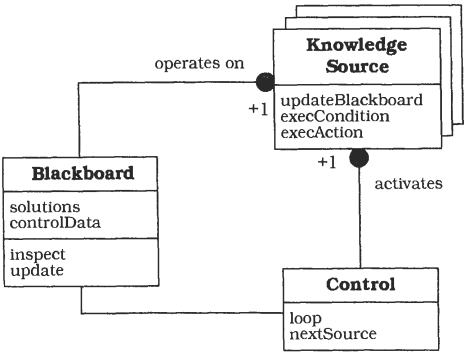
\includegraphics[width=0.6\textwidth]{figures/02-blackboard-1}
	\caption{Zusammenspiel der Blackboard Komponenten}
\end{figure}

\section{Consequences}
\begin{itemize}
    \pro{Experimentieren mit verschiedenen Algorithmen}
    \pro{Verschiedene Kontrollheuristiken können verknüpft werden}
    \pro{Unterstützt Wartbarkeit und Veränderbarkeit}
    \pro{Wiederverwendbare Wissensquellen}
    \pro{Fault Tolerance und Robustness}
    \con{Schwierig zu testen}
    \con{Keine gute Lösung garantiert}
    \con{Schwierig eine gute Kontrollstrategie zu entwickeln}
    \con{Tiefe Effizienz}
    \con{Hoher Entwicklungsaufwand}
    \con{Kein Support für Parallelität}
\end{itemize}

\section{Known Uses}
\begin{itemize}
	\item CRYSALIS (X-Ray Bilderkennung)
	\item HEARSAY-II (Spracherkennung)
	\item HASP/SIAP (Erkennung von gegnerischen U-Booten)
	\item TRICERO (Monitoring von Flugzeug Aktivitäten) 
\end{itemize}

\section{Relationships}
\begin{itemize}
	\item \textit{Keine} 
\end{itemize}

\section{Exam Questions}
\begin{itemize}
  \item Behauptung: dies ist eine Behauptung? (Lösung)
    \item Frage: Dies ist eine Frage? (Lösung)
\end{itemize}

\chapter{Model-View-Controller}

\section{Summary}
Das Model-View-Control-Pattern (MVC) teilt eine Applikation in drei Komponenten, wobei Programmlogik und Daten von der Präsentation getrennt werden. Ein Change-Progragation-Mechanismus sorgt dafür, dass die Daten zwischen den Schichten konsistent bleiben.
\section{Context}
Interaktive Applikationen mit einem flexiblen User-Interface.
\section{Problem}
User-Interfaces (UI) verursachen viel Arbeit. Wenn neue Features entwickelt werden, müssen dazu UIs entwickelt werden, ein Kunde möchte eine spezifische Änderung der Benutzerführung oder die Applikation muss auf eine andere Plattform mit einem anderen \textit{look and feel} portiert werden. 

Einem System die benötigte Flexibiltät zu geben, kann teuer und fehleranfällig werden, wenn das UI eng mit der Programmlogik verknüpft ist. Es kann dazu führen, dass verschiedene Softwaresysteme parallel gepflegt werden müssen, eines für jede UI-Implementation.

Folgende Forces beeinflussen die Lösungen zu solchen Problemen:
\begin{itemize}
	\item Die gleichen Informationen müssen auf verschiedene Weise präsentiert werden (z.B. Balken- oder Kuchendiagramm)
	\item Die Darstellung oder das verhalten einer Applikation müssen sofort auf veränderte Daten reagieren
	\item Änderungen am UI sollten einfach und sogar zur Laufzeit möglich sein
	\item Verschiedene \textit{look and feel} Standards oder eine Portierung des UIs sollten den Code der Kernfunktionalität der Applikation nicht beeinflussen
\end{itemize}

\section{Solution}
MVC teilt die Applikation in drei Bereiche: \textit{Verarbeitung}, \textit{Output} und \textit{Input}. 

Die \textbf{Model}-Komponente kapselt die Daten und Kernfunktionalität. Das Model ist unabhängig von spezifischen Datenrepräsentationen oder Eingabeverhalten

\textit{View}-Komponenten zeigen die Informationen dem Benutzer an. Eine View erhält die Daten vom Model. Zu einem Model können mehrere Views existieren

Jede View hat eine dazugehörige \textit{Controller}-Komponente. Controller wandeln den Input des Benutzers (Mausbewegungen, Mausklicks, Tastatureingaben) in Service Requests für das Model oder die View um. Der Benutzer interagiert mit dem System nur über Controller.

Diese Trennung ermöglicht es, für ein Model mehrere Views zu haben. Wenn nun der Benutzer über den Controller Daten im Model ändert, müssen alle anderen Views dieses Models diese Änderungen auch anzeigen. Deshalb benachrichtigt das Model alle Views über Änderungen. Dies wird durch das Publisher-Subscriber-Pattern gelöst.

Die nachfolgende Grafik zeigt den Zusammenhang zwischen Model, View und Controller:

\begin{figure}[H]
	\centering
	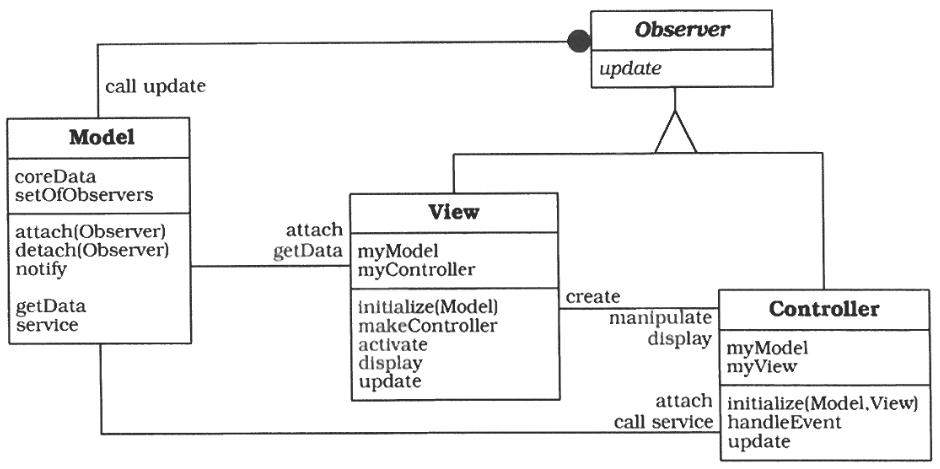
\includegraphics[width=0.8\textwidth]{figures/03-mvc-1}
	\caption{Zusammenhang zwischen MVC-Komponenten}
\end{figure}


\section{Consequences}
\begin{itemize}
    \pro{Mehrere Views für ein Model}
    \pro{Synchronisierte Views}
    \pro{Auswechselbare Views und Controller, sogar zur Laufzeit}
    \pro{Austauschbarkeit des \textit{look and feel}}
    \pro{Auf diesem Pattern kann ein Framework aufgebaut werden}
    \con{Erhöhte Komplexität}
    \con{Eine einzelne Aktion des Benutzers kann eine übermässige Anzahl Updates auslösen}
    \con{Controller und View sind sehr eng verzahnt, was deren einzelne Wiederverwertbarkeit erschwert}
    \con{Views und Controller sind stark an ein Model gekoppelt $\rightarrow$ Änderungen am Model erfordern Änderung an Views und Controller}
    \con{Ineffiziente Datendarstellung: Je nach Interface des Models müssen mehrere Requests gemacht werden, um das Interface aufzubauen}
\end{itemize}

\section{Known Uses}
\begin{itemize}
	\item \textbf{Smalltalk:} Das User Interface Framework in Smaltalk
	\item \textbf{MFC:} Die Document-View-Variation von MVC dient in C++ als Basis für Windows-Applikationen
	\item \textbf{ET++:} Das Applikations-Framework ET++ arbeitet auch mit einer Document-View-Variation
\end{itemize}

\section{Relationships}
\begin{itemize}
	\item Das \textit{Presentation-Abstraction-Control}-Pattern zeigt einen anderen Ansatz um das User Interface vom funktionalen Kern einer Applikation zu trennen.
\end{itemize}

\section{Exam Questions}
\begin{itemize}
  \item Behauptung: dies ist eine Behauptung? (Lösung)
    \item Frage: Dies ist eine Frage? (Lösung)
\end{itemize}

\chapter{Presentation-Abstraction-Control}

\section{Summary}
Das Presentation-Abstraction-Control (PAC) Pattern definiert eine Struktur für interaktive Software Systeme in Form einer Hierarchie von zusammenarbeitenden Agents. Jeder Agent ist dabei für einen spezifischen Teil der Funktionalität der Software zuständig. Ein Agent besteht aus den Komponenten Presentation, Abstraction und Control. Diese Unterteilung separiert den Mensch-Computer-Interaktions Aspekt des Agents von seinem funktionellen Kern und der Kommunikation mit anderen Agents.
\section{Context}
Entwicklung einer Interaktiven Applikation mit Einsatz von Agents.
\section{Problem}
Interaktive Systeme können oft als eine Sammlung von zusammenarbeitenden Agents gesehen werden. In solch einem System ist jeder Agent auf eine bestimmte Aufgabe spezialisiert, und alle Agents zusammen bilden das System. Folgende Forces haben einen Einfluss auf die Lösung:
\begin{itemize}
	\item Agents haben oft ihren eigenen State bzw. ihre eigenen Daten. Um zusammenarbeiten zu können brauchen die Agents einen Mechanismus zum Austausch von Daten, Messages und Events.
	\item Interaktive Agents bieten oft ihr eigenes Interface.
	\item Systeme entwickeln sich über die Zeit. Änderungen an einzelnen Agents oder das hinzufügen solcher sollte keinen Effekt auf das gesamte System haben.
\end{itemize}
\section{Solution}
Strukturierung der interaktiven Applikation als eine baumartige Hirarchie von PAC Agents, wobei es einen Top-Level Agent, mehrere Intermediate-Level Agents und noch mehr Bottom-Level Agents gibt. Jeder Agent ist abhängig von allen Agents auf einem höheren Level rauf bis zum Top-Level Agent. Im folgenden die Aufgaben der Level:
\paragraph{Top-Level Agent} Bietet den funktionellen Kern des Systems
\paragraph{Bottom-Level Agents} Repräsentieren in sich geschlossene semantische Konzepte auf denen User des Systems arbeiten können. 
\paragraph{Intermediate-Level Agents} Repräsentieren entweder Kombinationen oder Beziehungen zwischen Low-Level Agents. 
Ein Agent ist in die Komponenten Presentation, Abstraction und Control unterteilt. Die Presentation Komponente bietet das sichtbare Verhalten des PAC Agent. Von der Abstraction Komponente wird das Datenmodell verwaltet, sie bietet Funktionalität welche auf diesen Daten operiert. Die Control Komponente verbindet Presentation und Abstraction, und bietet zusätzlich Funktionalität die dem Agent ermöglicht mit anderen Agents zu kommunizieren.
\subsection{Structure}
Folgende Grafik zeigt die oben erwähnten drei Levels für eine Beispiel Applikation die als Informationssystem für Politische Wahlen dient. 
\begin{figure}[H]
	\centering
	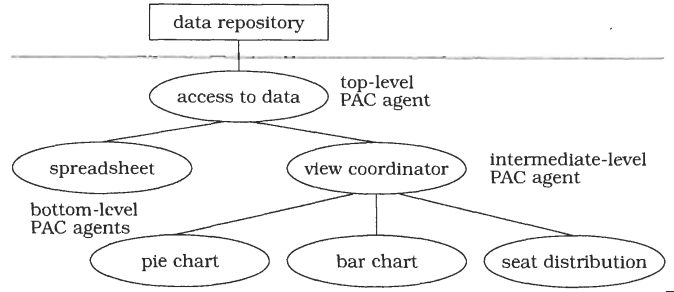
\includegraphics[width=0.6\textwidth]{figures/04-pac-1}
	\caption{PAC Level in einer Beispiel Applikation}
\end{figure}
Wie man sieht gibt es einen Top-Level PAC Agent. Dieser ist wie jeder Agent in die drei Komponenten unterteilt. Die Presentation Komponente hat auf diesem Level kaum Verantwortlichkeiten. Sie hat vieleicht UI Komponenten die von der gesamten Applikation verwendet werden, oder sie fällt ganz weg. 
Die Control Komponente auf diesem Level ermöglicht Lower-Level Agents auf die Services dieses Layers zuzugreifen, ausserdem koordiniert sie die Hierarchie der Agents und hält Informationen über die Interaktion des Users mit dem System.
Die Abstraction Komponente bietet in der Beispiel Applikation eine Schnittstelle zum darunter liegenden Daten Repository, es werden ausserdem Algorithmen zur Berechnung von Vorhersagen etc. hier implementiert. \\
Bottom-Level PAC Agents präsentieren auf der Presentation Komponente eine spezifische View der Daten, und bieten Zugriff auf alle Funktionen die ein User auf diesen tätigen kann. Die Abstraction Komponente ist ebenfalls für die Datenhaltung zuständig, allerdings sind hier keine anderen Agents davon abhängig. Die Control Komponente dient als Adapter zwischen Presentation und Abstraction, ausserdem kommuniziert Sie mit den höher gelegenen Agents. \\
Intermediate-Level PAC Agents können zwei verschiedene Rollen haben, composition oder coordination. In der composition Role führen sie die Bottom-Level Agents zu einer Abstraktion zusammen. In der coordination Role sind sie für die Konsistenz zwischen den Lower-Level Agents zuständig. 

\section{Consequences}
\begin{itemize}
    \pro{Separation of Concerns}
    \pro{Support for Change and Extention}
    \con{Erhöhte System Komplexität}
	\con{Komplexe Control Komponente}
	\con{Effizienz}
	\con{Anwendbarkeit}
\end{itemize}

\section{Known Uses}
\begin{itemize}
	\item Netzwerk Verkehr Management System
	\item Mobile Robot
\end{itemize}

\section{Relationships}
\begin{itemize}
	\item \textit{Model-View-Controller} 
\end{itemize}

\section{Exam Questions}
\begin{itemize}
  \item Behauptung: dies ist eine Behauptung? (Lösung)
    \item Frage: Dies ist eine Frage? (Lösung)
\end{itemize}

\chapter{Microkernel}

\section{Summary}
Das Micokernel Pattern wird bei Software Systemen angewendet, die sich an ändernde System Anforderungen anpassen können müssen. Es separiert einen aufs Minimum reduzierten Kern von zusätzlichen Funktionalitäten und Kunden spezifischen Teilen. Der Microkernel dient auch als Socket für diese Erweiterungen und er koordiniert ihre Zusammenarbeit.
\section{Context}
Entwicklung von mehreren Applikationen welche ähnliche Interfaces verwenden, welche auf der selben Grundfunktionalität aufbauen.
\section{Problem}
Software für ein Anwendungsgebiet zu entwickeln, welches mit einem breiten Spektrum von ähnlichen Standards und Technologien umgehen muss ist nicht einfach. Oft wird noch eine lange Lebenszeit gefordert, in welcher neue Technologien aufkommen und alte sich verändern. Das typische Beispiel für solche Software sind Betriebssysteme. Folgende Forces benötigen spezielle Aufmerksamkeit beim Design solcher Software:
\begin{itemize}
	\item Kontinuierliche Hardware und Software Evolution
	\item Einfache Portabilität, Erweiterbarkeit und einfache Integration von neuen Technologien
\end{itemize}

\section{Solution}
Das Microkernel Pattern schafft Abhilfe für oben erwähnte Probleme. Dabei werden die fundamentalen Services einer Applikationsplattform in eine Microkernel Komponente gepackt. Der Microkernel bietet anderen Komponenten die in separaten Prozessen laufen, die Möglichkeit miteinander zu kommunizieren. Er verwaltet ausserdem System weite Ressourcen, und er bietet Interfaces die anderen Komponenten Zugriff auf seine Funktionen bieten.
\subsection{Structure}
Das Microkernel Pattern definiert fünf Arten von teilnehmenden Komponenten, welche im folgenden kurz erklärt werden.
\paragraph{Microkernel} Der Microkernel repräsentiert die Hauptkomponente des Patterns. Er implementiert zentrale Services für die Kommunikation und Handhabung von Ressourcen. Alle anderen Komponenten bauen auf den Interfaces die der Microkernel für diese Services bietet, auf. Viele System spezifische Abhängigkeiten (Bsp. Hardware) sind im Microkernel vor den anderen Komponenten versteckt.
\paragraph{Internal Server} Internal Servers sind separate Komponenten welche die Funktionalität des Mikrokernels erweitern. Der Microkernel ruft die Funktionalität des Servers via Service Request auf. Internal Servers können also auch gewisse Abhängigkeiten zum darunterliegenden Software System haben. Ein Beispiel für ein Internal Server wären Grafikkarten Treiber für spezifische Modelle. Internal Servers können als Erweiterungen des Microkernels, welche nur bei Bedarf geladen werden und nur vom Microkernel zugreifbar sind, gesehen werden.
\paragraph{External Server} Als External Server wird eine Komponente bezeichnet, welche auf die Interfaces des Microkernels zugreift und darauf eine eigene View aufbaut. Externe Server laufen in separaten Prozessen und bieten selbst wiederum Interfaces an. Sie erhalten Service Requests über den Kommunikations Service des Microkernels.
\paragraph{Client} Ein Client ist eine Applikation die mit genau einem External Server in Bezug steht. Clients implementieren oft das Adapter Pattern um flexibler auf Änderungen am External Server reagieren zu können. \\
Das folgende Diagramm zeigt die statische Struktur eines Microkernel Systems mit den zuvor erläuterten Komponenten:
\begin{figure}[H]
	\centering
	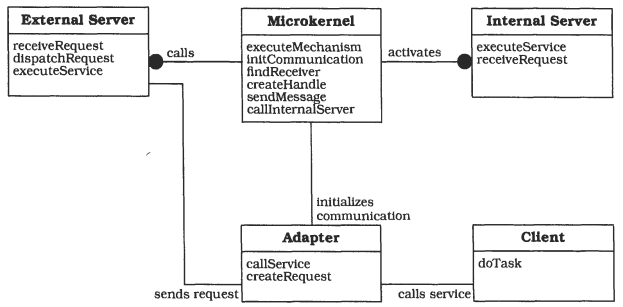
\includegraphics[width=0.7\textwidth]{figures/05-microkernel-1}
	\caption{Microkernel Struktur}
\end{figure}
\section{Consequences}
\begin{itemize}
    \pro{Portability}
    \pro{Flexibility and Extensibility}
    \pro{Separation of Policy and Mechanism}
    \pro{Scaleability}
    \pro{Reliability}
    \pro{Transparancy}
    \con{Performance}
    \con{Complexity of Design and Implementation}
\end{itemize}

\section{Known Uses}
\begin{itemize}
	\item Windows NT
	\item Chorus OS
	\item MKDE (Microkernel Database Engine)
\end{itemize}

\section{Relationships}
\begin{itemize}
	\item \textit{Broker Pattern}
	\item \textit{Reflection Pattern} 
	\item \textit{Layers Pattern}
\end{itemize}

\section{Exam Questions}
\begin{itemize}
  \item Behauptung: dies ist eine Behauptung? (Lösung)
    \item Frage: Dies ist eine Frage? (Lösung)
\end{itemize}

\chapter{Broker}

\section{Summary}
Das Broker Pattern kann verwendet werden, um verteilte Software Systeme zu strukturieren, welche durch Service-Aufrufe interagieren. Eine Broker-Komponente ist verantwortlich für die Koordination der Kommunikation. Das beinhaltet das Weiterleiten von Requests, sowie die Übermittlung von Resultaten und Exceptions.

\section{Context}
Ein verteiltes und möglicherweise heterogenes System mit unabhängigen kooperierenden Komponenten.

\section{Problem}
Wenn ein kompliziertes System aus einer Reihe miteinander interagierenden, losgelösten Komponenten geschaffen wird, anstelle einer monolithischen Applikation, erhöht dies die Flexibilität, Wartbarkeit und Veränderbarkeit. Durch die Partitionierung der Funktionalität in unabhängige Komponenten kann das System potentiell verteilt und skaliert werden.

Durch die Verteilung der Komponenten entsteht allerdings die Notwendigkeit einer Form von Interprozesskommunikation. Falls die Komponenten diese Kommunikation selbst übernehmen, entstehen dadurch Abhängigkeiten und Limitationen. Beispielsweise wird das System vom verwendeten Kommunikationsmechanismus abhängig.

Aus Sicht eines Entwicklers sollte es keinen Unterschied zwischen der Softwareentwicklung für ein verteiltes oder ein zentralisiertes Systems geben. Eine Applikation welche ein Objekt benutzt, sollte nur dessen Interface kennen. Details über die Implementation oder den physikalischen Ort sollten nicht bekannt sein. 

\medskip
Folgende Forces sind zu beachten:
\begin{itemize}
	\item Service-Aufrufe sollen \glqq location-transparent\grqq{} sein
	\item Komponenten müssen zur Laufzeit ausgetauscht, hinzugefügt und entfernt werden können
	\item Die Architektur soll System- und implementationsspezifische Details vor dem Benutzer vestecken
\end{itemize}

\section{Solution}
Führe eine Broker-Komponente ein um eine bessere Entkopplung von Server und Clients zu erreichen. Server registrieren sich beim Broker und stellen ihre Services durch Interfaces zur Verfügung. Clients greifen auf die Server zu, indem sie Requests an den Broker senden. Dieser leitet die Requests an den zuständigen Server weiter und übermittelt Resultate und allfällige Exceptions zurück an den Client.

\subsection{Structure}
Das Broker Pattern definiert sechs Arten von teilnehmenden Komponenten, welche im folgenden kurz erklärt werden.

\paragraph{Server}
Server implementieren Objekte welche ihre Funktionalität durch Interfaces zur Verfügung stellen. Diese Interfaces werden durch eine Interface Definition Language (IDL) oder durch einen binären Standard beschrieben.

Es werden folgende zwei Arten von Servern unterschieden:
\begin{itemize}
	\item Server welche Services für verschiedene Anwendungsbereiche anbieten
	\item Server welche eine spezifische Funktionalität für einen einzelnen Anwendungsbereich oder Aufgabe implementieren
\end{itemize}

\paragraph{Client}
Ein Client ist eine Applikation welche auf die Services von mindestens einem Server zugreift. Dieser Zugriff erfolgt über den Broker. Der Client muss nicht wissen wo sich der Server befindet.

Die Interaktion zwischen Client und Server basiert auf einem dynamischen Modell. Das bedeutet, dass ein Server auch als Client auftreten kann.

\paragraph{Broker}
Der Broker ist ein Messenger welcher verantwortlich ist für die Übertragung von Requests vom Client zum Server, sowie die Übertragung von Antworten und Exceptions zurück zum Client. Der Broker muss in der Lage sein, den Empfänger eines Requests anhand eines eindeutigen Identifiers zu ermitteln. 

Falls eine Anfrage für einen Server ankommt welcher nicht vom lokalen Broker verwaltet wird, muss die Anfrage an einen anderen Broker weitergeleitet werden. Broker müssen also auch untereinander kommunizieren können.

\paragraph{Client-side Proxy}
Ein Client-side Proxy ermöglicht ein zusätzliches Layer zwischen Client und Broker. Dieses zusätzliche Layer bietet Transparenz, indem ein entferntes Objekt für den Client als lokales Objekt dargestellt wird. Der Proxy kann dadurch Implementationsdetails vor dem Client verstecken wie die Kommunikation mit dem Broker und das Transformieren von Parametern und Resultaten.

\paragraph{Server-side Proxy}
Server-side Proxies sind grundsätzlich analog zu Client-side Proxies. Der Unterschied besteht darin dass sie sich zwischen Broker und Server befinden.

\paragraph{Bridge}
Bridges sind optionale Komponenten welche Implementationsdetails bei der Interoperation verschiedener Broker verstecken können. Sie kapseln dabei Netzwerk- oder Systemspezifische Daten. Eine Bridge vermittelt zwischen dem lokalen Broker und der Bridge eines entfernten Brokers.

\begin{figure}[H]
	\centering
	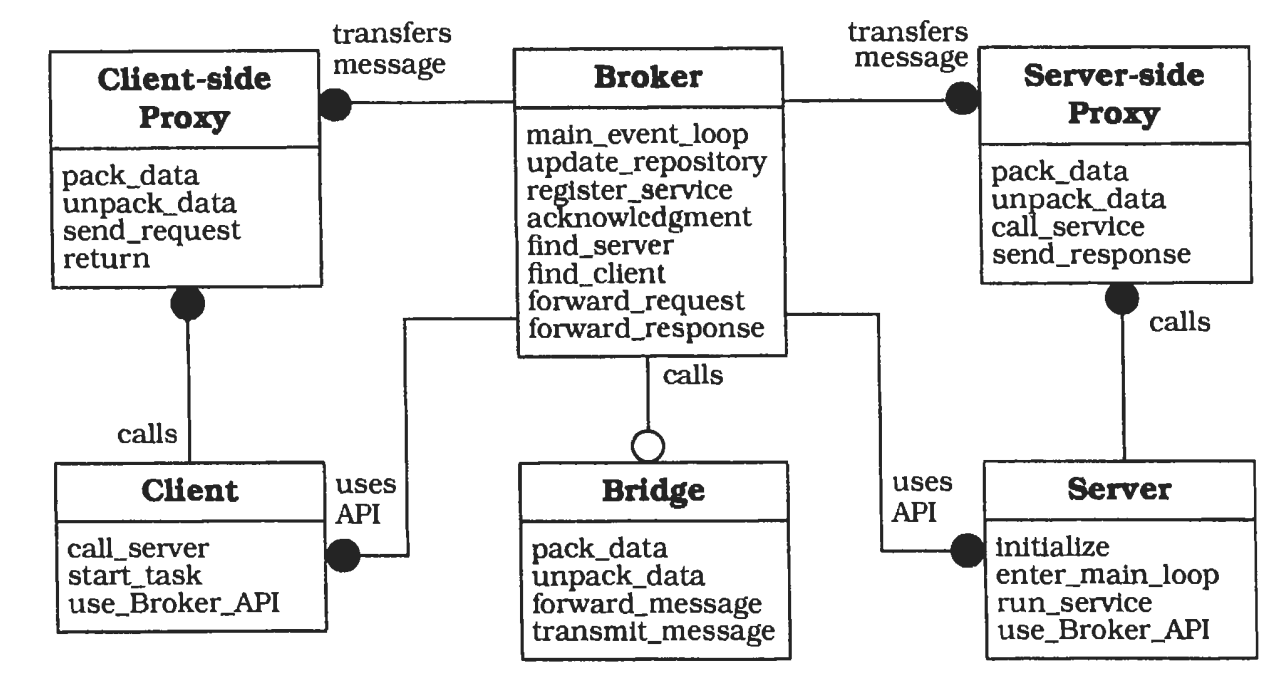
\includegraphics[width=0.8\textwidth]{figures/06-broker-1}
	\caption{Broker Struktur}
\end{figure}

\begin{figure}[H]
	\centering
	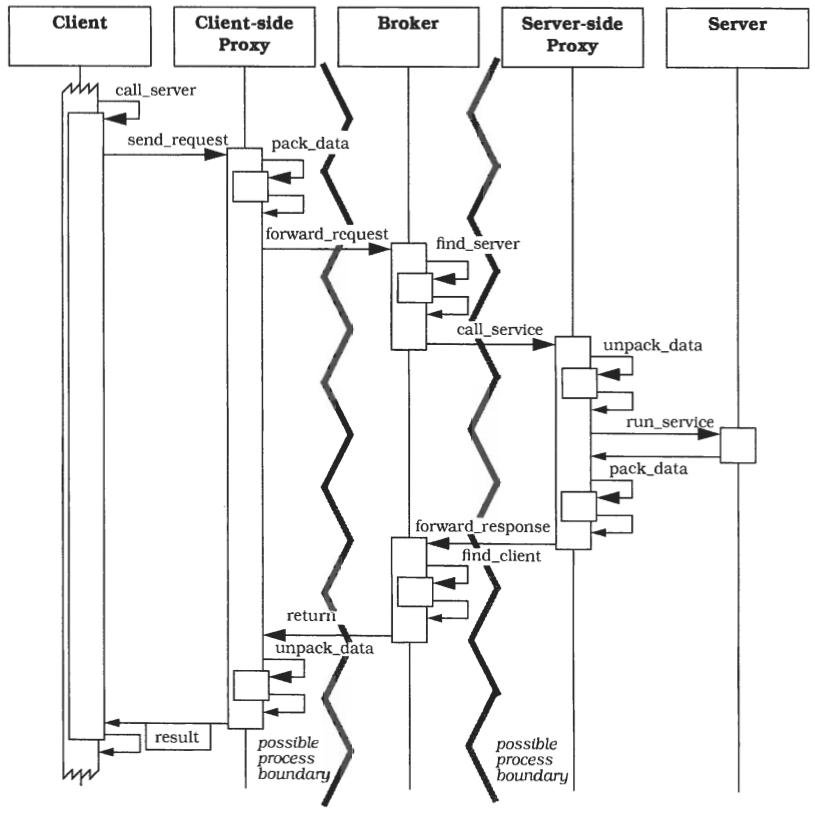
\includegraphics[width=0.8\textwidth]{figures/06-broker-2}
	\caption{Broker Sequenzdiagramm}
\end{figure}

\section{Variants}

\paragraph{Direct Communication Broker System}
In dieser Variante können Clients direkt mit dem Server kommunizieren. Der Broker teilt dem Client mit über welchen Kommunikationskanal der Server erreichbar ist.

\paragraph{Message Passing Broker System}
In dieser Variante stellen die Server keine Services zur Verfügung, sondern empfangen Messages und entscheiden anhand von deren Typ, was damit zu tun ist. Eine Message besteht dabei aus Rohdaten, sowie zusätzlichen Informationen welche den Typ, die Struktur und die Attribute der Message beschreiben.

\paragraph{Trader System}
Normalerweise wird ein Request zu einem einzigen eindeutig identifizierbaren Server weitergeleitet. In einem Trader System sind allerdings die Services und nicht die Server eindeutig identifizierbar. Ein Request kann somit an mehrere Server weitergeleitet werden, welche den gleichen Service implementieren.

\paragraph{Adapter Broker System}
In dieser Variante wird das Interface des Brokers gegenüber den Servern durch einen zusätzlichen Layer versteckt. Dadurch kann die Flexibilität erhöht werden. Der Adapter-Layer ist ein Teil des Brokers und ist verantwortlich für das Registrieren der Server und die Interaktion mit den Servern. Wenn mehr als ein Adapter angeboten wird, können damit verschiedene Strategien zur Granularität und dem Ort der Server unterstützt werden.

\paragraph{Callback Broker System}
Beim Ballback Broker System wird ein reaktives Kommunikationsmodell verwendet. Es wird dabei nicht zwischen Client und Server unterschieden. Wenn ein Event ankommt ruft der Broker die Callback-Methode derjenigen Komponente auf, welche registriert wurde auf den Event zu reagieren. Dieser Aufruf kann neue Events erzeugen welche wiederum den Broker dazu bringen können, weitere Callback-Methoden aufzurufen.

\section{Consequences}
\begin{itemize}
	\pro{Location Transparency}
	\pro{Changeability and extensibility of components}
	\pro{Portability of a Broker system}
	\pro{Interoperability between different Broker systems}
	\pro{Reusability}	
	\con{Restricted efficiency}
	\con{Lower fault tolerance}
\end{itemize}


\section{Known Uses}
\begin{itemize}
	\item CORBA
	\item IBM SOM/DSOM
	\item World Wide Web
	\item ATM-P
\end{itemize}

\section{Relationships}
\begin{itemize}
	\item \textit{Forwarder-Receiver Pattern}
	\item \textit{Proxy Pattern} 
	\item \textit{Client-Dispatcher-Server Pattern}
	\item \textit{Mediator design Pattern} 
\end{itemize}

\section{Exam Questions}
\begin{itemize}
	\item Behauptung: dies ist eine Behauptung? (Lösung)
    \item Frage: Dies ist eine Frage? (Lösung)
\end{itemize}

\clearpage
\vspace*{\fill}
\begin{center}
    { \huge \bfseries :wq }
\end{center}
\vfill
\clearpage


\end{document}
